% =========================================================================
%  AMR-Bench-mini: A Diagnostic Benchmark for Agentic Mechanistic AMR Reasoning
%
%  Target venue: GenBio @ ICML 2026 — short paper (4 pages)
%  Deadline:     2026-05-01 AOE
%
%  Built with the GenBio Overleaf template linked from the official CFP:
%      https://www.overleaf.com/read/dnjfbdnypxwn
% =========================================================================
\documentclass{article}

\usepackage{microtype}
\usepackage{graphicx}
\usepackage{booktabs}
\usepackage{hyperref}
\newcommand{\theHalgorithm}{\arabic{algorithm}}
\usepackage{icml2026}
\usepackage[T1]{fontenc}
\usepackage{xcolor}
\usepackage{amsmath}
\usepackage{tabularx}
\usepackage{tikz}
\usetikzlibrary{positioning,shapes.geometric}

\icmltitlerunning{AMR-Bench-mini}

\begin{document}
\twocolumn[
  \icmltitle{AMR-Bench-mini: A Diagnostic Benchmark for Agentic\\
  Mechanistic AMR Reasoning under Evidence Insufficiency}

  \begin{icmlauthorlist}
    \icmlauthor{Anonymous Authors}{anon}
  \end{icmlauthorlist}
  \icmlaffiliation{anon}{Anonymous Institution}
  \icmlcorrespondingauthor{Anonymous Author}{anon.email@domain.com}
  \icmlkeywords{AMR, agentic AI, benchmark, evidence sufficiency}
  \vskip 0.3in
]
\printAffiliationsAndNotice{}

\begin{abstract}
Frontier language-model agents have rapidly converged on a planner+tools+critic
architecture for biological reasoning, but it is unclear whether they reason
about \emph{evidence sufficiency} or merely pattern-match plausible mechanisms.
We introduce AMR-Bench-mini, a focused diagnostic benchmark for agentic
mechanistic antimicrobial-resistance (AMR) reasoning, scoped strictly to
retrospective evidence synthesis on \emph{Klebsiella pneumoniae}. The benchmark
pairs a 924-task corpus generated from public isolate metadata, genome
assemblies, laboratory AST, and pinned annotation outputs with two evaluation
splits: a balanced 50-task pilot and a 50-task hard diagnostic split organised
into seven category-level failure modes. We document an audit-and-fix loop
that lifts heuristic gold credibility from 71\,\% to 93\,\%, with four
disagreements where all three vendors converged against the heuristic gold. Three
frontier models (GPT-5.4, Gemini~3.1~Pro, Claude~Opus~4.7) score 82--88\,\% on
the pilot and 50--64\,\% on the hard split. All three converge on
$\sim$25\,\% accuracy on the abstention category, while contrastive-control
categories remain high descriptively. A pre-resolved CARD
ARO substrate-context tool injected into Gemini's prompt produces a
zero-percentage-point net effect on hard accuracy, with two gains and two
losses: substrate retrieval is necessary but not sufficient for
evidence-sufficiency reasoning.
\end{abstract}

\section{Introduction}
\label{sec:intro}

Agentic biology systems
\cite{coscientist,chemcrow,biomni,virtuallab,robin,saga,cocientist,txagent,fleming}
have converged on a recognisable template: a planner routes work through
domain tools, a memory holds intermediate results, and an optional critic
loop refines the answer. This template has been validated on chemistry
\cite{chemcrow}, CRISPR design \cite{biodiscoveryagent}, antibody
optimisation \cite{virtuallab}, and antibiotic discovery
\cite{saga,fleming}. Existing biology-agent benchmarks and evaluations
\cite{labbench,bixbench,biomni,scienceagentbench,bioplanner,astabench,genentech_agentic_compbio}
contain isolated AMR items, but no public benchmark targets agentic AMR
reasoning specifically.

The gap is not data: BV-BRC \cite{bvbrc}, CARD \cite{card}, AMRFinderPlus
\cite{amrfinder}, ResFinder, MEGARes \cite{megares}, and CRyPTIC are
extensive. The gap is task design under \emph{evidence insufficiency}.
Mechanistic AMR reasoning frequently requires the agent to recognise that
visible annotation evidence does \emph{not} deterministically explain an
observed clinical phenotype, and to propose a falsifiable hypothesis instead
of a plausible-sounding mechanism.

We make three contributions:

\begin{enumerate}\itemsep0.1em
\item \textbf{A diagnostic benchmark} (\S\ref{sec:bench}) of 924 mechanistic
AMR tasks (with paired 1{,}201 GenoPheno and 987 DBReconcile tracks) generated
from 60 public \emph{K.\,pneumoniae} isolates, with a balanced 50-task pilot
and a 50-task hard split organised into seven category-level failure modes,
including evidence insufficiency, substrate-specificity decoys,
intrinsic/acquired ontology, and hybrid mechanisms.
\item \textbf{An audit-and-fix methodology} (\S\ref{sec:audit}). A first-round
microbiologist audit on 31 stratified cards exposed five priority bugs in the
heuristic gold; after correction, a second round on 29 fresh cards reduced
the non-KEEP rate from 29\,\% to 7\,\%. Four further disagreements where all
three vendors agreed against the heuristic gold were adjudicated to the vendor
consensus.
\item \textbf{Cross-vendor invariance and a null tool result} (\S\ref{sec:results}).
Three frontier models score 50--64\,\% on the hard split with overlapping
Wilson 95\% confidence intervals; all three converge on $\sim$25\,\%
accuracy on the abstention category. Pre-resolving CARD ARO substrate
context into Gemini's prompt produces a zero-percentage-point net effect on
hard accuracy, with two gains and two losses, ruling out substrate retrieval
as the missing ingredient for evidence-sufficiency reasoning.
\end{enumerate}

\section{Benchmark construction}
\label{sec:bench}

\subsection{Scope and corpus}

The benchmark evaluates retrospective evidence synthesis only; clinical
treatment recommendation, wet-lab protocols, pathogen engineering, and novel
antibiotic design are explicitly out of scope, with outputs in those styles
scored as failures. The current corpus is 60 public \emph{K.\,pneumoniae}
isolates from BV-BRC \cite{bvbrc}, 60 paired FASTA assemblies, 1{,}410
laboratory AST records, and AMRFinderPlus \cite{amrfinder} and ResFinder
annotation outputs for every isolate. External tool versions and Docker
image digests are pinned in \texttt{outputs/provenance.json}
(AMRFinderPlus 4.2.7 / db 2026-03-24.1; ResFinder db 2.5.1).

The benchmark exposes three tracks: \textbf{GenoPheno}
(genotype$\rightarrow$phenotype with mechanism rationale),
\textbf{DBReconcile} (annotator-disagreement classification), and
\textbf{MechReason} (the headline track). MechReason asks for a five-layer
mechanistic explanation (genome, protein, mechanism, cell, phenotype)
plus a \texttt{mechanism\_class} drawn from a fixed 9-term vocabulary
that includes \texttt{insufficient\_evidence} as an explicit option for
cases where visible evidence cannot deterministically explain the AST
phenotype; such cases require a falsifiable hypothesis and a concrete
validation step. The MechReason corpus contains 924 tasks; this paper
focuses on two evaluation splits drawn from it.

\subsection{Audit-and-fix gold loop}
\label{sec:audit}

Heuristic gold labels were generated by a deterministic priority-ordered
mapping from gene-class evidence to mechanism class. We audited gold via two
stratified rounds (over-sampling \texttt{permeability\_loss},
\texttt{regulator\_loss\_of\_function}, and \texttt{insufficient\_evidence}).

\paragraph{Round 1 (n=31).} 22 KEEP / 5 OVERRIDE / 4 AMBIGUOUS. The audit
surfaced five systematic priority errors, including (i) regulator
loss-of-function being preferred over drug-specific efflux when the
substrate is tetracycline plus \emph{tet(A)}, (ii) cefoxitin resistance with
visible non-AmpC $\beta$-lactamases being mis-attributed to enzymatic
inactivation when porin-loss is the dominant mechanism, and (iii) a
substring-matching bug in $\beta$-lactamase family detection that mis-tagged
11 cefoxitin tasks. These were corrected in
\texttt{infer\_mechanism()} and the corpus was rebuilt.

\paragraph{Round 2 (n=29).} 27 KEEP / 1 OVERRIDE / 1 AMBIGUOUS. The non-KEEP
rate dropped from 29\,\% to 7\,\%. Hybrid carbapenem cases (ESBL
hyper-expression $+$ porin loss) were preserved with optional schema fields
\texttt{secondary\_mechanism\_classes} and \texttt{interaction\_type}
populated by the auditor.

\paragraph{Cross-vendor invariant disagreements.} Tri-vendor pilot
evaluation (\S\ref{sec:results}) flagged four cases where all three frontier
models from independent vendors agreed on a label \emph{against} the
heuristic gold: three \emph{fosA} tasks (heuristic
\texttt{intrinsic} $\rightarrow$ vendor consensus
\texttt{enzymatic\_inactivation}; \emph{fosA} is mechanistically a chromosomal
glutathione-S-transferase, with intrinsic acquisition status orthogonal to
mechanism class) and one ArmA hybrid amikacin task (heuristic
\texttt{enzymatic\_inactivation} $\rightarrow$ vendor consensus
\texttt{target\_modification} for the dominant 16S rRNA methyltransferase
contribution). We treat these as adjudicated overrides and report both
strict and adjudicated accuracies in every results table.

\subsection{Hard diagnostic split}
\label{sec:hardsplit}

The hard split is 50 tasks deterministically drawn from the corpus to stress
seven categorical failure modes; we summarise them tersely and refer the
reader to the released taxonomy document for full definitions.
\textbf{C1 hypothesisgen\_insufficient\_evidence} (\textit{n}=24) is the
abstention category: correct behaviour is to recognise that visible
wild-type \emph{tet(A)/oqxAB} is insufficient for tigecycline R without
regulator LoF or a tigecycline-active variant, that \emph{qnr} alone is
insufficient for clinical ciprofloxacin R without \emph{gyrA}/\emph{parC}
QRDR mutations or efflux hyper-expression, etc., and to output a
falsifiable hypothesis. \textbf{C2 intrinsic\_acquired\_ontology}
(\textit{n}=3): chromosomal \emph{fosA} cases that probe the vocabulary's
mechanism-vs-acquisition-status conflation. \textbf{C3
regulator\_lof\_vs\_direct\_efflux} (\textit{n}=2): cases where regulator
LoF is the dominant mechanism rather than the downstream pump.
\textbf{C4 hybrid\_porin\_beta\_lactamase} (\textit{n}=4): primary
permeability-loss + secondary $\beta$-lactamase carbapenem cases on a
single isolate. \textbf{C5 cefoxitin\_substrate\_decoy} (\textit{n}=10):
cefoxitin R with visible non-AmpC, non-carbapenemase $\beta$-lactamases
that are not expected to sufficiently explain cefoxitin resistance; gold is
\texttt{permeability\_loss}.
\textbf{C6 drug\_specificity\_positive\_control} (\textit{n}=4): positive
controls paired by isolate to C1 tigecycline cases (same gene profile,
drug differs). \textbf{C7 cefoxitin\_true\_hydrolysis\_control}
(\textit{n}=3): one KPC, one NDM, and one CMY/AmpC representative that
genuinely hydrolyse cefoxitin.

\section{Results}
\label{sec:results}

\subsection{Setup}

We evaluate three frontier models (GPT-5.4, Gemini~3.1~Pro Preview,
Claude~Opus~4.7) under a single shared scaffolded system prompt, with
provider-native APIs. Claude is run via the Anthropic Message Batches API at
50\,\% list-price discount; OpenAI and Gemini run live. Each task receives a
single attempt with no retries, no chain-of-thought scratchpad, and no tool
calls (the tool experiment in \S\ref{sec:tool} explicitly augments only the
prompt context, not the inference loop). Scoring is composite: a task is
correct only when (i) \texttt{mechanism\_class} matches gold, (ii) the
required-gene family appears in the model's evidence list (or the prediction
is \texttt{insufficient\_evidence}), and (iii) all five mechanistic layers
are populated.

\begin{table*}[t]
\centering
\caption{Composite accuracy with Wilson 95\% confidence intervals. Strict =
heuristic gold; adjudicated = post-audit gold with the four invariant
overrides applied. CIs are computed only when subgroup $n \geq 10$.}
\label{tab:headline}
\small
\begin{tabular}{llcc}
\toprule
\textbf{Split} & \textbf{Model} & \textbf{Strict} & \textbf{Adjudicated} \\
\midrule
Balanced pilot ($n=50$)  & GPT-5.4         & 74.0\,\% [60.4, 84.1] & 82.0\,\% [69.2, 90.2] \\
Balanced pilot ($n=50$)  & Gemini 3.1 Pro  & 80.0\,\% [67.0, 88.8] & \textbf{88.0\,\%} [76.2, 94.4] \\
Balanced pilot ($n=50$)  & Claude Opus 4.7 & 78.0\,\% [64.8, 87.2] & 86.0\,\% [73.8, 93.0] \\
\midrule
Hard diagnostic ($n=50$) & GPT-5.4         & 44.0\,\% [31.2, 57.7] & 50.0\,\% [36.6, 63.4] \\
Hard diagnostic ($n=50$) & Gemini 3.1 Pro  & 58.0\,\% [44.2, 70.6] & \textbf{64.0\,\%} [50.1, 75.9] \\
Hard diagnostic ($n=50$) & Claude Opus 4.7 & 54.0\,\% [40.4, 67.0] & 60.0\,\% [46.2, 72.4] \\
\bottomrule
\end{tabular}
\end{table*}

\subsection{Headline numbers}

Adjudication adds 6--8\,pp uniformly across vendors
(Table~\ref{tab:headline}). The hard split drops all three by roughly
20\,pp relative to the balanced pilot; Wilson intervals overlap but
Gemini~3.1~Pro is consistently strongest. On the balanced pilot, Gemini's
failure set is a strict subset of GPT-5.4's (10 invariant, 3 GPT-only,
0 Gemini-only). On the hard split under adjudicated gold, this becomes
17 tri-vendor-invariant failures (all C1), 1 GPT+Gemini shared failure
(C1), 7 GPT-only failures (6 C5, 1 C1), 3 Claude-only failures (mixed),
and 0 Gemini-only failures. The residual cross-vendor failure set is
therefore concentrated entirely on evidence-insufficiency cases
(Figure~\ref{fig:per-category}).

\begin{figure*}[t]
\centering
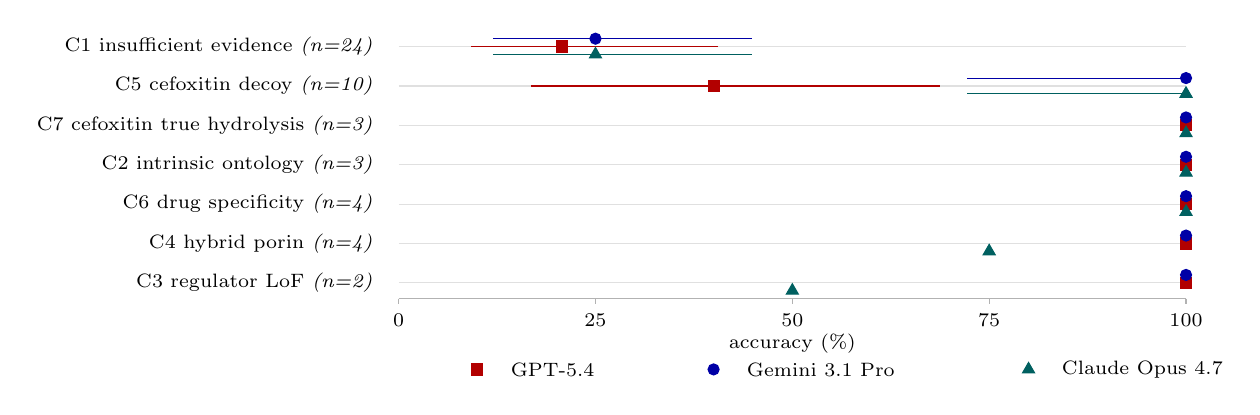
\begin{tikzpicture}[
    font=\footnotesize, x=10cm, y=0.5cm,
    gptmark/.style    ={fill=red!70!black,   draw=red!70!black,  rectangle, minimum size=4pt, inner sep=0pt},
    gemmark/.style    ={fill=blue!65!black,  draw=blue!65!black, circle,    minimum size=4pt, inner sep=0pt},
    claudemark/.style ={fill=teal!75!black,  draw=teal!75!black, regular polygon, regular polygon sides=3, minimum size=5pt, inner sep=0pt},
  ]
  % ---- axis frame: x in [0,1] = accuracy 0..100% ; y rows top-to-bottom ----
  \def\rA{6} \def\rB{5} \def\rC{4} \def\rD{3} \def\rE{2} \def\rF{1} \def\rG{0}
  \draw[black!30] (0,\rG-0.4) -- (1,\rG-0.4);
  \foreach \x/\lab in {0/0, 0.25/25, 0.5/50, 0.75/75, 1/100} {
    \draw[black!30] (\x,\rG-0.4) -- (\x,\rG-0.55);
    \node[anchor=north, font=\scriptsize] at (\x,\rG-0.55) {\lab};
  }
  \node[anchor=north, font=\scriptsize] at (0.5,\rG-1.05) {accuracy (\%)};

  % ---- horizontal guide lines + row labels ----
  \foreach \y/\lab/\n in {\rA/{C1 insufficient evidence}/24, \rB/{C5 cefoxitin decoy}/10, \rC/{C7 cefoxitin true hydrolysis}/3, \rD/{C2 intrinsic ontology}/3, \rE/{C6 drug specificity}/4, \rF/{C4 hybrid porin}/4, \rG/{C3 regulator LoF}/2} {
    \draw[black!12] (0,\y) -- (1,\y);
    \node[anchor=east, font=\scriptsize] at (-0.02,\y) {\lab\ \textit{(n=\n)}};
  }

  % ---- C1: Wilson CIs (n=24, k=5,6,6) ----
  \draw[red!70!black]  (0.092,\rA) -- (0.405,\rA); \node[gptmark]    at (0.208,\rA) {};
  \draw[blue!65!black] (0.120,\rA+0.20) -- (0.449,\rA+0.20); \node[gemmark]    at (0.250,\rA+0.20) {};
  \draw[teal!75!black] (0.120,\rA-0.20) -- (0.449,\rA-0.20); \node[claudemark] at (0.250,\rA-0.20) {};

  % ---- C5: Wilson CIs (n=10) — GPT 4/10, Gem 10/10, Claude 10/10 ----
  \draw[red!70!black]  (0.168,\rB) -- (0.687,\rB); \node[gptmark]    at (0.40,\rB) {};
  \draw[blue!65!black] (0.722,\rB+0.20) -- (1.00,\rB+0.20); \node[gemmark]    at (1.00,\rB+0.20) {};
  \draw[teal!75!black] (0.722,\rB-0.20) -- (1.00,\rB-0.20); \node[claudemark] at (1.00,\rB-0.20) {};

  % ---- C7: point estimates only (n=3); all 3/3 ----
  \node[gptmark]    at (1,\rC) {};
  \node[gemmark]    at (1,\rC+0.20) {};
  \node[claudemark] at (1,\rC-0.20) {};

  % ---- C2 intrinsic ontology (n=3): all 3/3 adjudicated ----
  \node[gptmark]    at (1,\rD) {};
  \node[gemmark]    at (1,\rD+0.20) {};
  \node[claudemark] at (1,\rD-0.20) {};

  % ---- C6 drug specificity (n=4): all 4/4 ----
  \node[gptmark]    at (1,\rE) {};
  \node[gemmark]    at (1,\rE+0.20) {};
  \node[claudemark] at (1,\rE-0.20) {};

  % ---- C4 hybrid porin (n=4): GPT 4/4, Gem 4/4, Claude 3/4 ----
  \node[gptmark]    at (1,\rF) {};
  \node[gemmark]    at (1,\rF+0.20) {};
  \node[claudemark] at (0.75,\rF-0.20) {};

  % ---- C3 regulator LoF (n=2): GPT 2/2, Gem 2/2, Claude 1/2 ----
  \node[gptmark]    at (1,\rG) {};
  \node[gemmark]    at (1,\rG+0.20) {};
  \node[claudemark] at (0.50,\rG-0.20) {};

  % ---- legend below ----
  \def\lY{-2.2}
  \node[gptmark]    at (0.10,\lY) {}; \node[anchor=west, font=\scriptsize] at (0.13,\lY) {GPT-5.4};
  \node[gemmark]    at (0.40,\lY) {}; \node[anchor=west, font=\scriptsize] at (0.43,\lY) {Gemini 3.1 Pro};
  \node[claudemark] at (0.80,\lY) {}; \node[anchor=west, font=\scriptsize] at (0.83,\lY) {Claude Opus 4.7};
\end{tikzpicture}
\vspace{0.6em}
\caption{Hard-split per-category accuracy under adjudicated gold. Markers
are point estimates; horizontal whiskers are Wilson 95\% CIs (drawn only
where $n \geq 10$). C1 (insufficient evidence) is the only subgroup where
all three vendors fall to ${\sim}25\%$, with intervals strictly below
those of C5 and below every contrastive-control point estimate
($\geq 75\%$).}
\label{fig:per-category}
\vspace{-0.6em}
\end{figure*}

\subsection{Tri-vendor abstention failure (C1)}

Figure~\ref{fig:per-category} breaks the hard split by category. Twenty of the
fifty hard-split tasks fail across all three vendors: 17 in C1
(\texttt{insufficient\_evidence}) and 3 in C2
(\texttt{intrinsic\_acquired\_ontology}). The C2 invariant failures are the
\emph{fosA} cases adjudicated in \S\ref{sec:audit}; under the adjudicated
gold all three vendors solve them, leaving the residual cross-vendor failure
set concentrated entirely in C1. The 95\% Wilson CI for C1 accuracy is
[9.2, 40.5] for GPT and [12.0, 44.9] for both Gemini and Claude; this is
the only categorical subgroup with $n \geq 10$ besides C5 (\textit{n}=10),
and it falls strictly below the C5 interval ([72.2, 100.0] for the two
saturating vendors) and below every contrastive-control point estimate
($\geq 75\%$). We read this as a calibration failure that is
\emph{model-invariant within current frontier-model knowledge}: the same
visible-evidence pattern repeatedly fails to register as insufficient across
three independent vendors.

\subsection{Tool intervention is not the fix}
\label{sec:tool}

To test whether the C1 failure is a knowledge-retrieval gap, we built a
deterministic CARD ARO substrate-lookup module
(\texttt{src/amr\_bench/tools/card\_substrate.py}) that, for every visible
gene in a task, injects the canonical AMR Gene Family, Drug Class coverage,
and Resistance Mechanism from CARD into the prompt as a markdown-formatted
substrate-context block, before the model sees the task JSON. We chose the
strongest model (Gemini~3.1~Pro) for this experiment because (i) GPT-5.4's
gain would conflate substrate-knowledge patching with calibration testing,
and (ii) Gemini was already at 100\,\% on the C5 substrate-decoy category
without tools, so any change on C1 isolates the calibration question
cleanly.

The result is a striking null: \emph{adjudicated} hard-split accuracy is
\textbf{32/50 with substrate context, identical to 32/50 without}. Two
gains and two losses cancel. Gains: C1 \texttt{kp\_000603} (TMP/SMX) and
\texttt{kp\_000872} (tigecycline), both
\texttt{efflux}$\rightarrow$\texttt{insufficient\_evidence}. Losses:
C1 \texttt{kp\_000569} (tigecycline), correct abstention $\rightarrow$
\texttt{efflux}; and C6 \texttt{kp\_000778} (tetracycline,
\emph{tet(A)}+\emph{oqxAB}), correct \texttt{efflux} $\rightarrow$
spurious abstention. The two losses are diagnostic: the CARD card for
\emph{oqxA/B} legitimately lists tetracycline alongside tigecycline, and
the model under substrate context anchors on the breadth of the listing
in both directions --- abstaining when efflux is correct and invoking
efflux when abstention is correct. Substrate context is, in other words,
\emph{bidirectionally persuasive}, the opposite of the calibration
property C1 requires. Pre-resolving substrate biology --- the most
natural retrieval intervention --- is necessary but not sufficient for
evidence-sufficiency reasoning.

\section{Limitations}

The current pilot is single-species (\emph{K.\,pneumoniae}) and modest in
isolate count (60). Hard-split rare classes ($n \leq 5$) cannot support
population-level claims and are reported as descriptive controls only;
collapsing them into a generic ``rare-mechanism'' bucket would obscure the
specific reasoning failure each was constructed to expose. Heuristic gold
remains a partial signal even after the audit loop; we therefore report
strict and adjudicated accuracies in every table and ship the
pre-adjudication snapshot for independent re-scoring. AST labels are
retrospective and inherit the testing standards of their source records.
Per-run token counts are logged to enable downstream cost calculation
against current published prices, which we do not assert.

\section{Reproducibility}

Every model run writes \texttt{raw\_outputs.jsonl} alongside a manifest
recording the SHA-16 of the frozen task subset, the SHA-16 of every prompt
template, the command line, the model and provider, and provider-reported
token usage; this lets the strict-vs-adjudicated rescoring be re-run against
new gold without re-querying the API. Annotator versions are pinned by
Docker RepoDigest in \texttt{outputs/provenance.json}. The CARD substrate
lookup, the audit loop, the hard-split builder, the headline table, and the
tool comparison are each one self-contained script. Code, data, gold
snapshots, and full per-run artifacts are released under the project
repository; no inference is required to reproduce any number reported in
this paper.

% =========================================================================
\bibliographystyle{icml2026}
\bibliography{refs}
% =========================================================================
\end{document}
